

\section{État de l'art}
\label{repl:sec:stateoftheart}

Cette section commence par décrire le schéma de réplication optimiste de
séquences -- un document pouvant être représenté par une séquence de caractères
(cf. §\ref{repl:subsec:optimistic}).  Ensuite, cette section passe en revue deux
familles d'approches appartenant à la réplication optimiste des séquences : les
transformées opérationnelles (cf. §\ref{repl:subsec:ot}) et les structures de
données répliquées sans conflits (cf. §\ref{repl:subsec:crdts}). Cette section
s'attache particulièrement à cette dernière famille et en détaille les
approches.

\subsection{Réplication optimiste de séquences}
\label{repl:subsec:optimistic}

\begin{figure}
  \begin{center}
    
\begin{tikzpicture}[scale=1.2]

  \newcommand\X{30pt};
  \newcommand\Y{30pt};
  
  \draw[->](0pt,   0pt)--(10*\X,   0pt);
  \draw[->](0pt, -1*\Y)--(10*\X, -1*\Y);
  \draw[->](0pt, -2*\Y)--(10*\X, -2*\Y);
  
  \draw[fill=black](0pt, 0pt) node[anchor=east]{réplique 1 }circle(2pt);
  \draw[fill=black](0pt, -1*\Y) node[anchor=east]{réplique 2 }circle(2pt);
  \draw[fill=black](0pt, -2*\Y) node[anchor=east]{réplique 3 }circle(2pt);

  \draw(\X,2pt)--node[anchor=south]{[WERTY]}( \X,   -2pt);
  \draw(\X,2 -1*\Y)--node[anchor=south]{[WERTY]}(\X,-2 -1*\Y);
  \draw(\X,2 -2*\Y)--node[anchor=south]{[WERTY]}(\X,-2 -2*\Y);
  \small
  \draw(3* \X,2pt)--node[anchor=north]
  {(a) \textsc{insert}(Q, 0) \DARKBLUE{\textbf{produit} $resultat$}}(3 * \X,   -2pt);
%  \draw(3* \X,2 -2*\Y)--node[anchor=north]{\textsc{delete}(\DARKBLUE{\textbf{0}})}(3 * \X,-2 -2*\Y);
  \normalsize

  \draw(3* \X,2pt)--node[anchor=south]{[QWERTY]}(3 * \X,   -2pt);
%  \draw(2* \X,2 -1*\Y)--node[anchor=south]{[ ]}(2* \X,-2 -1*\Y)
%  \draw(3* \X,2 -2*\Y)--node[anchor=south]{[ERTY]}( 3 * \X,-2 -2*\Y);

  \small
  \draw[->, dashed] (5*\X, 0pt) -- (15+7*\X, -1*\Y);
  \draw[->, dashed] (5*\X, 0pt)
  node[anchor = south west]{(b) \DARKBLUE{\textbf{dissémine}} $resultat$} -- (7*\X, -2*\Y);


  \draw (15+ 7*\X, 2-1*\Y) -- (15+ 7*\X, -2-1*\Y)
  node [anchor=north]{(c)};
  \draw (7*\X, 2-2*\Y) -- (7*\X, -2-2*\Y)
  node [anchor=north]{(c) \DARKBLUE{\textbf{intègre}} $resultat$ };
  \normalsize

%  \draw[->, dashed] (5*\X, -2*\Y) -- (7*\X,  0*\Y)
%  node[anchor=south]{\textsc{delete}(\DARKBLUE{\textbf{0}})};
%  \normalsize
%  \draw[->, dashed] (5*\X, -2*\Y) -- (7*\X, -1*\Y);

  \draw(9*\X, 2 -0*\Y)--node[anchor=south]{[QWERTY]}(9*\X,-2 -0*\Y);
  \draw(9*\X, 2 -1*\Y)--node[anchor=south]{[QWERTY]}(9*\X,-2 -1*\Y);
  \draw(9*\X, 2 -2*\Y)--node[anchor=south]{[QWERTY]}(9*\X,-2 -2*\Y);


%%  \draw(9*\X, 2 -0*\Y)--node[anchor=south]{[QWERTY]}(9*\X,-2 -0*\Y);
%%  \draw(9*\X, 2 -1*\Y)--node[anchor=south]{[QWERTY]}(9*\X,-2 -1*\Y);
%%  \draw(9*\X, 2 -2*\Y)--node[anchor=south]{[QWERTY]}(9*\X,-2 -2*\Y);


%%  \draw[fill=white, very thick]
%%  (0*\X, 0*\Y) node{$p_1$} +(-5pt,-5pt) rectangle +(5pt,5pt);
%%  \draw[->](-5+\X, 5+2*\Y)to[out=120,in=30](0pt,5+2*\Y); %% 6 -> 7
\end{tikzpicture}
    \caption[Étapes de la réplication
    optimiste]{\label{repl:fig:optimisticsteps} Les 3 étapes de la réplication
      optimiste.}    
  \end{center}
\end{figure}

La réplication optimiste~\cite{demers1987epidemic, johnson1975maintenance,
  ladin1992providing, saito2005optimistic} de séquence est un paradigme de
réplication où chaque éditeur possède une réplique locale du document.  Un
document est toujours disponible et réactif aux changements effectués. En effet,
comme l'illustre la figure~\ref{repl:fig:optimisticsteps},
\begin{inparaenum}[(a)]
\item une opération de modification est directement exécutée sur la réplique
  locale de la séquence.  La modification produit un résultat qui
\item est disséminé aux autres serveurs hébergeant une réplique.
\item Le serveur exécute -- ou \emph{intègre} -- le résultat reçu.
\end{inparaenum}
% Grâce à $\textsc{insert}(Q, 0)$, un résultat est
% produit puis disséminé aux deux autres répliques. L'intrégation de ce résultat

\noindent La réplication optimiste fait l'hypothèse d'une dissémination fiable
où tous les serveurs reçoivent toutes les modifications afin que toutes les
répliques convergent vers un état équivalent. Ainsi, après réception et
intégration du $resultat$, les trois répliques de la
figure~\ref{repl:fig:optimisticsteps} contiennent la même séquence
\texttt{QWERTY}.

Sun et al.~\cite{sun1998achieving} déclarent que l'édition collaborative temps
réel nécessite un système préservant les trois propriétés CCI :

%\begin{itemize}
\paragraph{Convergence.} Les répliques ayant reçues les mêmes opérations
convergent vers un état identique. Par exemple, la
figure~\ref{repl:fig:optimisticsteps} montre que les répliques peuvent avoir des
états temporairement divergent. En revanche, après réception et intégration du
résultat de l'opération d'insertion, les trois répliques convergent vers une
séquence identique.

\noindent La convergence fait l'objet de critère de cohérence à part entière
tels que la cohérence à terme~\cite{bailis2013eventual}, ou la cohérence forte à
terme~\cite{shapiro2011conflict}. Ces critères de cohérence sont très faibles
mais ont beaucoup de succès ces dernières années avec, par exemple, les bases de
données réparties~\cite{dynamo, riak, cassandra, mongodb}.
% Malheureusement, ces critères sont trop expressifs : l'état de convergence
% n'est pas spécifié. Par exemple, ils permettent aux répliques de converger
% vers un état arbitraire n'ayant aucun lien avec les modifications apportées
% par les participants. À ce titre, ces critères seuls sont insuffisants pour
% l'édition collaborative.

\begin{figure}
  \begin{center}
    
\begin{tikzpicture}[scale=1.2]

  \newcommand\X{30pt};
  \newcommand\Y{30pt};
  
  \draw[->](0pt,   0pt)--(10*\X,   0pt);
  \draw[->](0pt, -1*\Y)--(10*\X, -1*\Y);
  \draw[->](0pt, -2*\Y)--(10*\X, -2*\Y);
  
  \draw[fill=black](0pt, 0pt) node[anchor=east]{réplique 1 }circle(2pt);
  \draw[fill=black](0pt, -1*\Y) node[anchor=east]{réplique 2 }circle(2pt);
  \draw[fill=black](0pt, -2*\Y) node[anchor=east]{réplique 3 }circle(2pt);

  \draw(\X,2pt)--node[anchor=south]{[WERTY]}( \X,   -2pt);
  \draw(\X,2 -1*\Y)--node[anchor=south]{[WERTY]}(\X,-2 -1*\Y);
  \draw(\X,2 -2*\Y)--node[anchor=south]{[WERTY]}(\X,-2 -2*\Y);
  \small
  \draw(3* \X,2pt)--node[anchor=north]
  {\textsc{insert}(Q, 0)}(3 * \X,   -2pt);
%  \draw(3* \X,2 -2*\Y)--node[anchor=north]{\textsc{delete}(\DARKBLUE{\textbf{0}})}(3 * \X,-2 -2*\Y);
  \normalsize

  \draw(3* \X,2pt)--node[anchor=south]{[QWERTY]}(3 * \X,   -2pt);
%  \draw(2* \X,2 -1*\Y)--node[anchor=south]{[ ]}(2* \X,-2 -1*\Y)
%  \draw(3* \X,2 -2*\Y)--node[anchor=south]{[ERTY]}( 3 * \X,-2 -2*\Y);

  \small
  \draw[->, dashed] (4*\X, 0pt) -- (4.5*\X, -1*\Y);
  \draw[->, dashed] (4*\X, 0pt) to[out=25,in=155] (7.5*\X, 0pt)
  to[out=-40,in=95] (8.2*\X, -2*\Y);
  
  \draw(5.5*\X, 2-1*\Y)node[anchor=south]{\normalsize[WERTY]}--(5.5*\X, -2-1*\Y)
  node[anchor=north]{\small\textsc{delete}(0)};

  \draw[->, dashed] (6.5*\X, -1*\Y) -- (7*\X, -0*\Y);
  \draw[->, dashed] (6.5*\X, -1*\Y) -- (7*\X, -2*\Y);

  \draw[->, dashed, color=darkblue] (7*\X, -2*\Y) to[out=-45,in=-135]
  node[anchor=north]{\DARKBLUE{\textbf{attend}}} (8.5*\X, -2*\Y);

  \normalsize

%  \draw[->, dashed] (5*\X, -2*\Y) -- (7*\X,  0*\Y)
%  node[anchor=south]{\textsc{delete}(\DARKBLUE{\textbf{0}})};
%  \normalsize
%  \draw[->, dashed] (5*\X, -2*\Y) -- (7*\X, -1*\Y);

  \draw(9*\X, 2 -0*\Y)--node[anchor=south]{[WERTY]}(9*\X,-2 -0*\Y);
  \draw(9*\X, 2 -1*\Y)--node[anchor=south]{[WERTY]}(9*\X,-2 -1*\Y);
  \draw(9*\X, 2 -2*\Y)--node[anchor=south]{[WERTY]}(9*\X,-2 -2*\Y);


%%  \draw(9*\X, 2 -0*\Y)--node[anchor=south]{[QWERTY]}(9*\X,-2 -0*\Y);
%%  \draw(9*\X, 2 -1*\Y)--node[anchor=south]{[QWERTY]}(9*\X,-2 -1*\Y);
%%  \draw(9*\X, 2 -2*\Y)--node[anchor=south]{[QWERTY]}(9*\X,-2 -2*\Y);


%%  \draw[fill=white, very thick]
%%  (0*\X, 0*\Y) node{$p_1$} +(-5pt,-5pt) rectangle +(5pt,5pt);
%%  \draw[->](-5+\X, 5+2*\Y)to[out=120,in=30](0pt,5+2*\Y); %% 6 -> 7
\end{tikzpicture}
    \caption[Exemple de respect des relations
    causales]{\label{repl:fig:causality}Exemple de respect des relations
      causales entre deux opérations.}
  \end{center}
\end{figure}

\paragraph{Causalité.} Si une opération précède une autre
opération~\cite{lamport1978time}, alors l'intégration de cette première
opération précède l'intégration de la seconde opération.  La causalité
contraint l'ordre d'intégration des opérations. Ainsi, une opération dépendante
d'une autre opération effectuée avant se trouve forcément intégrée à sa suite.
La figure~\ref{repl:fig:causality} montre un exemple où, sur la réplique 3,
l'intégration de l'opération de suppression doit attendre l'arrivée de
l'opération d'insertion pour supprimer le caractère \texttt{Q}.


% C'est une manière de forcer l'exécution correcte de cette première opération
% : le contexte d'exécution est le même que sur la réplique d'origine donc le
% résultat est le même.  Malheureusement, capturer toutes les relations
% causales s'avère coûteux~\cite{charronbost1991concerning}. Pour chaque
% participant ayant jamais effectué une modification sur le document, une
% valeur entière doit être conservée dans un vecteur. Ce vecteur indique les
% opérations visibles lors de l'exécution de cette opération.  De même que
% pour la convergence, baser l'édition collaborative seulement sur un ordre
% causal ne fonctionne pas : les opérations concurrentes n'ont pas de
% comportement défini.

\paragraph{Intention.} L'effet observé sur le document lors de la génération
d'une opération doit être également observé lors de son intégration.  Dans
l'exemple de la figure~\ref{repl:fig:causality}, la cible originelle de la
suppression sur la réplique 2 est le caractère \texttt{Q}. Par conséquent, ce
caractère doit être supprimé lors de l'intégration de l'opération, et nul autre
caractère.

% malgré l'
% interférence d'opérations concurrentes.  Lorsque les définitions des
% propriétés de convergence et de causalité font consensus,

\noindent L'intention des opérations d'une séquence demeure difficile à
formaliser dans le cas général. L'effet d'une opération doit respecter le plus
possible sa spécification séquentielle~\cite{bieniusa2012brief}. La
spécification séquentielle d'une séquence inclut deux opérations : \og insérer
l'élément $e$ à la position $i$ dans la séquence \fg et \og supprimer l'élément
à la position $i$ dans la séquence \fg. L'intention semble donc liée à la
position des éléments dans la séquence. Contre cette intuition, nous soutenons
qu'une séquence se définie plus simplement par un ordre dense sur ses éléments :
les éléments sont ordonnés et il est toujours possible d'insérer un élément
entre deux autres éléments. Les opérations usuelles d'insertion et de
suppression se traduisent par une transformation de position dans la séquence
vers un ordre dense.

\begin{definition}[Spécification séquentielle d'une séquence]
  Soit une série d'opérations $H$ produisant la séquence
  $s(H) = \{p_1,\, p_2 \ldots p_k\}$ avec $p_{1..k} \in \mathcal{P}$ où
  $\mathcal{P}$ est un ensemble muni d'un ordre
  dense $(\mathcal{P},\,<_\mathcal{P})$ tel que : \\
  $\forall p\in\mathcal{P},\, p_\vdash <_\mathcal{P} p <_\mathcal{P} p_\dashv $
  \hfill et \ \
  $p_\vdash <_\mathcal{P} p_1 <_\mathcal{P} p_2 <_\mathcal{P} \ldots
  <_\mathcal{P} p_k <_\mathcal{P} p_\dashv$.
  
  \noindent L'insertion d'un élément $e$ en position $i$ dans la séquence $s(H)$
  est définie de la façon suivante :
  \begin{equation}
    s(H \cup \textsc{insert}(i,\, e)) \rightarrow s(H) \cup 
    \begin{cases}
      \{p,\, p_\vdash <_\mathcal{P} p <_\mathcal{P} p_\dashv \} & i = 0 \wedge |s(H)| = 0\\
      \{p,\, p_\vdash <_\mathcal{P} p <_\mathcal{P} p_1 \} & i = 0 \wedge |s(H)|>0\\
      \{p,\, p_k <_\mathcal{P} p <_\mathcal{P} p_\dashv \} & i = k\\
      \{p,\, p_i <_\mathcal{P} p <_\mathcal{P} p_{i+1} \} & sinon
    \end{cases}
  \end{equation}

  \noindent La suppression de l'élément en position $i$ dans la séquence $s(H)$
  est définie de la façon suivante :
  \begin{equation}
    s(H \cup \textsc{delete}(i)) \rightarrow s(H) \setminus \{ p_i \}
  \end{equation}
\end{definition}

%\end{itemize}

Nous distinguons la complexité spatiale de la réplique, et la complexité en
communication sur les messages, la complexité temporelle d'une opération
exécutée localement, la complexité temporelle de l'intégration d'une opération
reçue.

\noindent Parmi ces complexités, la complexité en communication est la plus
critique et doit être sous-linaire pour passer à l'échelle. En ce qui concerne
les complexités temporelles, il est plus important d'améliorer l'intégration que
la génération car chaque opération locale effectuée conduit à $N$ intégrations,
où $N$ est le nombre de répliques.  Les opérations étant atomiques, leur
exécution est bloquante vis-à-vis des autres opérations. Un temps d'exécution
trop long constitue un danger pour l'édition en temps réel.

Le reste de cette section présente les approches appartenant à la réplication
optimiste de séquences : les approches à transformées opérationnelles (cf.
§\ref{repl:subsec:ot}) et les approches à structure de données proposant des
opérations commutatives (cf. §\ref{repl:subsec:crdts}).

\subsection{Transformées opérationnelles}
\label{repl:subsec:ot}

Les approches basées sur les transformées opérationnelles
(OT)~\cite{sun1998operational, sun2009contextbased} sont les plus anciennes. Les
opérations locales d'insertion et de suppression proposées possèdent une
signature correspondant exactement à la signature commune des séquences :
$\textsc{insert}(element,$ $position)$ et $\textsc{delete}(position)$. Lors de
la réception d'une opération, ses arguments sont ajustés afin qu'ils
s'appliquent à l'état courant de la réplique malgré les opérations effectuées et
intégrées en concurrence. Cette phase d'intégration nécessite l'examen des
opérations concurrentes afin d'en compenser les effets sur la séquence.

% En d'autres termes, le résultat d'une opération locale est l'opération
% elle-même. En revanche, son intégration nécessite l'examen des opérations
% concurrentes afin de compenser les changements sur l'ordre des éléments lors de
% son exécution locale.

\begin{figure}
  \centering
  
\begin{tikzpicture}[scale=1.2]

  \newcommand\X{30pt};
  \newcommand\Y{30pt};
  
  \draw[->](0pt,   0pt)--(10*\X,   0pt);
  \draw[->](0pt, -1*\Y)--(10*\X, -1*\Y);
  \draw[->](0pt, -2*\Y)--(10*\X, -2*\Y);
  
  \draw[fill=black](0pt, 0pt) node[anchor=east]{réplique 1 }circle(2pt);
  \draw[fill=black](0pt, -1*\Y) node[anchor=east]{réplique 2 }circle(2pt);
  \draw[fill=black](0pt, -2*\Y) node[anchor=east]{réplique 3 }circle(2pt);

  \draw(\X,2pt)--node[anchor=south]{[WERTY]}( \X,   -2pt);
  \draw(\X,2 -1*\Y)--node[anchor=south]{[WERTY]}(\X,-2 -1*\Y);
  \draw(\X,2 -2*\Y)--node[anchor=south]{[WERTY]}(\X,-2 -2*\Y);
  \small
  \draw(3* \X,2pt)--node[anchor=north]{\textsc{insert}(Q, 0)}(3 * \X,   -2pt);
  \draw(3* \X,2 -2*\Y)--node[anchor=north]{\textsc{delete}(\DARKBLUE{\textbf{0}})}(3 * \X,-2 -2*\Y);
  \normalsize

  \draw(3* \X,2pt)--node[anchor=south]{[QWERTY]}(3 * \X,   -2pt);
%  \draw(2* \X,2 -1*\Y)--node[anchor=south]{[ ]}(2* \X,-2 -1*\Y)
  \draw(3* \X,2 -2*\Y)--node[anchor=south]{[ERTY]}( 3 * \X,-2 -2*\Y);

  \draw[->, dashed] (5*\X, 0pt) -- (7*\X, -1*\Y);
  \draw[->, dashed] (5*\X, 0pt) -- (7*\X, -2*\Y);

  \small
  \draw[->, dashed] (5*\X, -2*\Y) -- (7*\X,  0*\Y)
  node[anchor=south]{\textsc{delete}(\DARKBLUE{\textbf{1}})};
  \normalsize
  \draw[->, dashed] (5*\X, -2*\Y) -- (7*\X, -1*\Y);

  \draw(9*\X, 2 -0*\Y)--node[anchor=south]{[QERTY]}(9*\X,-2 -0*\Y);
  \draw(9*\X, 2 -1*\Y)--node[anchor=south]{[QERTY]}(9*\X,-2 -1*\Y);
  \draw(9*\X, 2 -2*\Y)--node[anchor=south]{[QERTY]}(9*\X,-2 -2*\Y);


%%  \draw(9*\X, 2 -0*\Y)--node[anchor=south]{[QWERTY]}(9*\X,-2 -0*\Y);
%%  \draw(9*\X, 2 -1*\Y)--node[anchor=south]{[QWERTY]}(9*\X,-2 -1*\Y);
%%  \draw(9*\X, 2 -2*\Y)--node[anchor=south]{[QWERTY]}(9*\X,-2 -2*\Y);


%%  \draw[fill=white, very thick]
%%  (0*\X, 0*\Y) node{$p_1$} +(-5pt,-5pt) rectangle +(5pt,5pt);
%%  \draw[->](-5+\X, 5+2*\Y)to[out=120,in=30](0pt,5+2*\Y); %% 6 -> 7
\end{tikzpicture}
  \caption[Exemple de transformées opérationnelles] {\label{repl:fig:otexample}
    Exemple de scénario impliquant des transformées opérationnelles. L'opération
    de suppression du premier caractère sur la réplique 3 est transformée afin
    de supprimer le second caractère sur les autres répliques.}
\end{figure}

La figure~\ref{repl:fig:otexample} illustre le principe de fonctionnement des
approches basées sur OT sur un scénario impliquant une séquence répliquée. Dans
cet exemple, les répliques sont toutes initialisées avec la séquence
\texttt{WERTY}. Ensuite, tandis que la première réplique insère le caractère
\texttt{Q} en tête de séquence pour obtenir \texttt{QWERTY}, la troisième
réplique supprime son premier caractère correspondant au \texttt{W}. Lorsque la
réplique 1 reçoit cette dernière opération de suppression, elle est interprétée
comme une opération dont le contexte d'exécution n'avait pas encore intégré
l'insertion du caractère \texttt{Q}. Le décalage d'une position vers la droite
de chaque caractère n'avait donc pas encore été intégré. Par conséquent,
l'argument de l'opération voit sa cible changée au second caractère :
\texttt{W}.  Réciproquement, la réplique 3 intègre l'insertion de la réplique 1
: l'insertion et la suppression sont détectées concurrentes, toutefois aucune
transformation n'est nécessaire. À terme, les répliques convergent vers la
séquence \texttt{QERTY}. % Sans transformation, la réplique 1 aurait obtenu la
% séquence \texttt{WERTY} et la propriété de convergence du système aurait été
% bafouée.

% Dans le cadre de l'édition de textes, en plus des usuelles opérations
% d'insertion et de suppression, OT fournit des opérations ciblant les chaînes de
% caractères telles que le déplacement, ou le couper -- coller. Toutefois,
% l'analyse de correction nécessite d'examiner chaque couple d'opérations ainsi
% que leurs arguments. En conséquence, lors de l'écriture du
% papier~\cite{imine2003proving}, peu d'approches étaient réellement
% correctes. \TODO{Keep it or not?}

Dans les approches OT décentralisées~\cite{sun2009contextbased}, chaque client
est aussi un serveur hébergeant une réplique de la séquence. Deux problèmes
apparaissent : 

\paragraph{Coût de la détection.} Chacune de ces entités doit être en mesure
d'effectuer les transformations d'elle-même. Parmi les pré-requis à cette tâche
figure le mécanisme de détection de concurrence. En effet, retrouver le contexte
d'exécution revient à transformer l'opération reçue contre toutes celles qui ont
été intégrées sans en avoir connaissance. Cependant, chaque message doit
transporter un vecteur d'horloges (\emph{vector clock})~\cite{lamport1978time}
ou de contexte pour chaque opération. Par conséquent, la complexité en
communication est au minimum linéaire par rapport au nombre de répliques.  De
plus, ces vecteurs et leur opération associée sont ensuite sauvegardés dans un
historique. La complexité spatiale est au minimum linéaire selon les deux
dimensions : nombre de répliques et nombre d'opérations.

\paragraph{Répartition des temps d'exécution.} La génération d'une opération
s'exécute en temps constant. Cependant, son intégration s'exécute en temps
quadratique par rapport au nombre d'opérations concurrentes à l'opération
intégrée. Cette répartition des coûts d'opération est malheureuse car 1
opération locale efficace correspond à $N$ exécutions distantes potentiellement
lentes, où $N$ est le nombre de répliques recevant l'opération.

Pour ces raisons, les approches OT décentralisées ne passent pas à l'échelle. A
contrario, dans un environnement bien maîtrisé, où les opérations arrivent très
rapidement à un groupe raisonnable de participants, ces approches décentralisées
sont extrêmement efficaces~\cite{mehdi2014merging}.

\subsection{Structure de données répliquée sans conflits}
\label{repl:subsec:crdts}

Les structures de données répliquées sans conflits
(\emph{CRDTs}\footnote{\emph{Conflict-free Replicated Data
    Types}})~\cite{shapiro2011comprehensive, shapiro2011conflict} appartiennent
au schéma de réplication optimiste. Ces approches sont basées sur des structures
de données abstraites fournissant des opérations dont les résultats commutent
par nature. Les répliques convergent donc vers un état identique même en cas de
concurrence. Contrairement aux approches OT, les opérations concurrentes n'ont
pas besoin d'être détectées. Les CRDTs s'affranchissent donc de la nécessité de
joindre un vecteur d'horloges à chaque opération. Sans cette contrainte, les
CRDTs ont l'opportunité de passer à l'échelle. Contrairement aux approches OT,
la signature des opérations est différente des séquences \og classiques \fg et
correspond à l'intention telles que nous la définissons où une séquence est un
ensemble d'éléments muni d'un ordre dense : les éléments sont ordonnés et il est
toujours possible d'insérer un élément entre deux autres éléments. Par exemple,
\og insérer l'élément $e$ à la position $i$ \fg devient \og insérer l'élément
$e$ entre l'élément en position $i$ et l'élément en position $i+1$ \fg.

Pour fonctionner , les CRDTs pour séquences surchargent chaque élément d'une
métadonnée nommée identifiant. Les identifiants, uniques et immuables,
permettent d'assurer un ordre total (convergence) sur les éléments tout en
respectant un ordre dense (intention) établi lors de l'exécution locale de
l'insertion. Par exemple, si l'élément $e$ est inséré entre l'élément $p$ et
l'élément $q$, alors il n'existe aucune réplique où l'intégration de cette
opération résulterait en une séquence où $e$ n'est pas placé -- directement ou
non -- entre $p$ et $q$.  Si $p$ ou $q$ n'existe(nt) plus car supprimé(s), alors
l'intégration de $e$ doit tout de même respecter l'ordre dense établi lors de
l'insertion de $p$ et $q$. Par exemple, si $o$ précède $p$ dans la séquence mais
que $p$ est supprimé, alors $o$ précède -- directement ou non -- l'élément $e$.

Selon la manière dont les identifiants sont générés, nous distinguons deux types
d'approches : les approches recourant à des marqueurs nommés \og pierre tombales
\fg (cf. §\ref{repl:subsubsec:tombstones}); et les approches générant des
identifiants dont la taille varie (cf. §\ref{repl:subsubsec:variable}).

\subsubsection{Pierres tombales}
\label{repl:subsubsec:tombstones}

Une \og pierre tombale \fg est une marque laissée après la suppression d'un
élément indiquant qu'un jour, celui-ci a existé à cet emplacement. Ces marques
sont cachées à l'utilisateur : les caractères disparaissent du document mais
existent toujours dans la structure répliquée.

%% L'impact sur les performances à
%% l'intégration des opérations en reste néanmoins présent.

\paragraph{WOOT~\cite{oster2006data} :} WOOT est le premier représentant
historique des CRDTs pour séquences suivi par deux extensions
\textbf{WOOTO~\cite{weiss2007wooki}} et
\textbf{WOOTH~\cite{ahmed2011evaluating}}. Dans cette approche chaque
identifiant fait référence aux identifiants voisins à l'insertion.  Lorsqu'ils
sont rassemblés, les identifiants peuvent être ordonnés grâce à un diagramme de
Hasse. Toutefois, cet ordonnancement requiert des deux bornes adjacentes
qu'elles soient
\begin{inparaenum}[(i)]
\item déjà intégrées et
\item toujours présentes.
\end{inparaenum}
%D'où les suppressions réelles impossibles.

\begin{figure}
  \centering
  
\begin{tikzpicture}[scale=1.1]

\newcommand\X{ 40pt}
\newcommand\Y{ 30pt}

\draw[fill=white](0 * \X, 0 * \Y) node{$\vdash$}+(-5pt,-5pt)rectangle+(5pt,5pt);
\draw[fill=white](7 * \X, 0 * \Y) node{$\dashv$}+(-5pt,-5pt)rectangle+(5pt,5pt);

\draw[fill=white](1 * \X, 1 * \Y) node{\textbf{Q}}+(-5pt,-5pt)rectangle+(5pt,5pt);
\draw[fill=white](2 * \X, 1 * \Y) node{\textbf{W}}+(-5pt,-5pt)rectangle+(5pt,5pt);

\draw[fill=white](1 * \X, 0 * \Y) node{\textbf{A}}+(-5pt,-5pt)rectangle+(5pt,5pt);
\draw[fill=white, draw=darkblue](2 * \X, 0 * \Y)
node{\DARKBLUE{\textbf{Z}}}+(-5pt,-5pt)rectangle+(5pt,5pt);
\draw[fill=white, draw=darkblue](3 * \X, 0 * \Y)
node{\DARKBLUE{\textbf{E}}}+(-5pt,-5pt)rectangle+(5pt,5pt);
\draw[fill=white](4 * \X, 0 * \Y) node{\textbf{R}}+(-5pt,-5pt)rectangle+(5pt,5pt);
\draw[fill=white](5 * \X, 0 * \Y) node{\textbf{T}}+(-5pt,-5pt)rectangle+(5pt,5pt);
\draw[fill=white](6 * \X, 0 * \Y) node{\textbf{Y}}+(-5pt,-5pt)rectangle+(5pt,5pt);

\draw[thick](-5+1*\X, -5+0*\Y)--(5+1*\X, 5+0*\Y);
\draw[thick](-5+1*\X, 5+0*\Y)--(5+1*\X, -5+0*\Y);

\draw[thick, color=darkblue](-5+2*\X, -5+0*\Y)--(5+2*\X, 5+0*\Y);
\draw[thick, color=darkblue](-5+2*\X, 5+0*\Y)--(5+2*\X, -5+0*\Y);

\draw[->](5+1*\X,-5+0*\Y)to[out=-45,in=-135](-5+7*\X, -5+0*\Y);
\draw[->](5+2*\X,-5+0*\Y)to[out=-45,in=-135](-5+7*\X, -5+0*\Y);
\draw[->](5+3*\X,-5+0*\Y)to[out=-45,in=-135](-5+7*\X, -5+0*\Y);
\draw[->](5+4*\X,-5+0*\Y)to[out=-45,in=-135](-5+7*\X, -5+0*\Y);
\draw[->](5+5*\X,-5+0*\Y)to[out=-45,in=-135](-5+7*\X, -5+0*\Y);
\draw[->](5+6*\X,-5+0*\Y)to[out=-45,in=-135](-5+7*\X, -5+0*\Y);

\draw[<-](5+0*\X, 0*\Y)--(-5+1*\X, 0*\Y);
\draw[<-, color=darkblue](5+1*\X, 0*\Y)--(-5+2*\X, 0*\Y);
\draw[<-, color=darkblue](5+2*\X, 0*\Y)--(-5+3*\X, 0*\Y);
\draw[<-](5+3*\X, 0*\Y)--(-5+4*\X, 0*\Y);
\draw[<-](5+4*\X, 0*\Y)--(-5+5*\X, 0*\Y);
\draw[<-](5+5*\X, 0*\Y)--(-5+6*\X, 0*\Y);

\draw[->](1*\X,5+1*\Y)to[out=50,in=130](3*\X, 5+0*\Y);
%\draw[->](2*\X,5+1*\Y)to[out=45,in=135](3*\X, 5+0*\Y);
\draw[->](5+2*\X, 1*\Y)--(-5+3*\X, 5+0*\Y);

\draw[<-](0*\X, 5+0*\Y)--(-5+1*\X, 1*\Y);
\draw[<-](5+1*\X, 1*\Y)--(-5+2*\X, 1*\Y);


\end{tikzpicture}
  \caption[Diagramme de Hasse dans WOOT]
  {\label{repl:fig:wootexample}Le diagramme de Hasse du modèle WOOT représentant
    la séquence \texttt{QWERTY}. Bien que supprimé, le caractère \texttt{Z} est
    indispensable au bon ordonnancement de la séquence.}
\end{figure}

\noindent La figure~\ref{repl:fig:wootexample} illustre la nécessité de
conserver les pierres tombales. Elle montre le diagramme de Hasse généré lors du
scénario suivant. Tout d'abord, un utilisateur écrit \texttt{AZERTY}. Ensuite,
les deux premiers caractères sont supprimés afin d'être remplacés par les
caractères \texttt{QW}. La séquence finale est \texttt{QWERTY}. Toutefois, les
identifiants ne sont pas modifiables, et l'identifiant du caractère \texttt{E}
référence l'identifiant de \texttt{Z}, lui-même référençant l'identifiant de
\texttt{A}. Par conséquent, supprimer complètement les identifiants de
\texttt{A} et/ou de \texttt{Z} revient à rendre l'identifiant de \texttt{E} non
positionnable, et tout ceux qui en dépendent par transitivité.

\noindent Même si le document peut apparaître vide, la structure répliquée contient
tous les éléments ayant été insérés depuis sa création. Cette croissance
monotone de la structure impacte négativement l'intégration des opérations qui
devient moins efficace. Du reste, la complexité en communication est optimale
puisque seul un identifiant de taille constante doit être envoyé par opération.

\paragraph{Causal tree~\cite{grishchenko2010deep} :} Cette approche caractérise
explicitement les relations causales grâce à une représentation sous forme
d'arbre. Ainsi, chaque opération est accompagnée de l'identifiant de la dernière
opération observée. En parcourant l'arbre et en appliquant les opérations, la
séquence peut être retrouvée. Toutefois, les identifiants sont des vecteurs
d'horloges dont la taille croît linéairement avec le nombre de participants. De
plus, il est nécessaire de conserver tous les nœuds de cet arbre causal au cas
où une opération y ferait référence. Cette approche garantie la réception
causale comme le prescrit la cohérence CCI~\cite{sun1998achieving}. Cependant,
elle n'est pas adaptée aux contextes où le groupe d'éditeurs est grand.

\paragraph{Partial persistent sequence~\cite{wu2010partial} :} Cette approche
définit les identifiants dans l'ensemble des nombres rationnels auxquels est
ajoutée une limite quant à leur précision. Hélas, cette limite contraint la
taille maximale que peut atteindre un document. Sans cette troncature,
l'approche serait susceptible d'appartenir à l'autre famille de CRDTs pour
séquence.

\paragraph{Replicated growable array~\cite{roh2011replicated} :} Cette structure
représente la séquence sous forme de liste supportant les opérations
concurrentes. Une table de hachage apporte un accès rapide aux éléments grâce à
leurs identifiants. Les éléments incluent une référence au voisin qu'ils
précèdent lors de leur insertion. Toutefois, pour ne jamais briser la chaîne
ainsi construite, les éléments supprimés sont cachés et restent présents dans la
structure. Une variante sous forme d'arbre a récemment été
proposée~\cite{attiya2016specification}. Tout comme pour WOOT, la mémoire locale
consommée par la réplique est monotone croissante. Les performances des
opérations se dégradent progressivement à chaque insertion.

\paragraph{String-wise~\cite{yu2012stringwise} :} Cette approche cible
principalement les chaînes de caractères pouvant être subdivisées lors
d'opérations jusqu'à devenir une série de caractères. Les identifiants
référencent alors les chaînes adjacentes à l'insertion ainsi que les autres
éléments de la chaînes si subdivision il y a. Le nombre d'identifiants générés
s'en trouve diminué. Cependant, de la même manière que pour les approches
précédentes, les références empêchent à la structure répliquée de se débarasser
des éléments supprimés. La complexité spatiale de l'approche est monotone
croissante et linéaire par rapport au nombre d'insertions et de
subdivisions. Les performances des opérations en sont impactées négativement.

% \paragraph{DiCE~\cite{conway2014language} :} Cet éditeur concentre
% principalement ses efforts sur les garanties de confluence de la
% séquence. Chaque identifiant référence le voisin qu'il précède à
% l'insertion. L'ordre des éléments est alors fonction de ces relations de
% positionnement relatif, et de causalité.

Pour préserver l'ordre dense défini lors de l'exécution locale de l'insertion,
toutes ces approches génèrent des identifiants qui référencent au moins l'un
des identifiants adjacent. Il devient impossible de supprimer un élément de la
structure répliquée sans mettre en danger l'ordre dense à préserver. Ainsi, les
suppressions conservent tous les éléments, qu'ils soient supprimés ou non du
document.  Un document peut être vide bien que la séquence répliquée possède des
milliers d'éléments cachés. La mémoire consommée par ces approches croît au
moins linéairement par rapport au nombre d'insertions faites dans la séquence. Plus
problématique : cette croissance est monotone.  Les pierres tombales dégradent à
jamais les performances de l'intégration des opérations où l'ordre des éléments
doit être retrouvé.

Purger la structure de données des éléments cachés est une solution potentielle
aux dégradations de performances. Un mécanisme de ramasse-miettes
réparti~\cite{abdullahi1998garbage} permet de nettoyer une structure de données
en vidant de la mémoire les objets qui ne sont plus accessibles par le
programme, ni localement ni à distance. Ainsi, supprimer réellement un élément
de la séquence revient à s'interroger : \og Est-ce que
\begin{inparaenum}[(i)]
\item toutes les répliques ont supprimé l'élément et
\item tous les éléments référençant l'élément supprimé ont été intégrés
  localement ?
\end{inparaenum}\fg Cela va sans dire qu'il est difficile d'apporter une réponse
à ces deux questions. D'autant plus lorsque les répliques ne sont pas
perpétuellement accessibles. Core-nebula~\cite{letia2009crdts} propose de
contraindre la topologie du réseau afin de rendre la prise de décision
possible. Ainsi, un cœur décisionnel prend en charge les choix de suppression
réelle des objets.  Ce cœur décisionnel est restreint à un sous-ensemble de
membres du réseaux toujours accessibles. Les décisions peuvent alors être prises
de manière fiable. Le reste des participants se conforme à ces décisions au
risque de perdre certaines de leurs modifications. Cette re-centralisation
expose le système aux problèmes de confidentialité, de censure, de propriété, de
passage à l'échelle et de tolérance aux défaillances.
 
Un autre famille de CRDTs existe pour le type séquence dont le bon
fonctionnement ne nécessite pas de référencer directement d'autres
identifiants. Cela évite l'usage des pierres tombales mais pose le problème de
la complexité spatiale des identifiants.

\subsubsection{Identifiants de taille variable}
\label{repl:subsubsec:variable}

Contrairement aux approches basées sur les pierres tombales, certains CRDTs
génèrent des identifiants ne référençant pas d'autres identifiants. Par
conséquent, ces identifiants sont indépendants : leur intégration ne nécessite
pas l'intégration d'autres identifiants. Ces identifiants ont une taille
variable définie à la génération~\cite{andre2013supporting,
  preguica2009commutative, weiss2009logoot}.  Ainsi, les identifiants sont
toujours uniques et immuables une fois générés, mais leur structure est une
liste de valeurs encodant la position relative de l'élément par rapport aux
positions relatives des éléments adjacents à son insertion. Ces identifiants
sont directement créés dans un ensemble muni d'un ordre total pour assurer la
convergence, et muni d'un ordre dense pour assurer l'intention. À ce titre, ces
approches constituent une implémentation directe de notre spécification
séquentielle des séquences.

% Contrairement aux approches basées sur les pierres tombales, ces identifiants
% sont indépendents : leur intégration ne dépend pas des autres identifiants. À ce
% titre, les suppressions ne se contentent pas de masquer les éléments mais les
% retirent entièrement de la structure. En revanche, la liste de valeurs
% constituant les identifiants est susceptible de grandir, et par là même, de
% diminuer les performances du système.

\paragraph{Logoot~\cite{weiss2010collaborative, weiss2009logoot,
    weiss2010logootundo} :} Ce CRDT représente la séquence sous forme de liste
d'identifiants. Chacun des identifiants est une liste de triples notée
$id = [t_1,\,t_2,\,\ldots,\,t_k]$ où $t_k=\langle p_k,\,s_k,\,c_k \rangle$ où
$p_k$ est un entier positif, $s_k$ est un identifiant unique de site, et $c_k$
est un compteur local au site $s_k$. Un ordre lexicographique est utilisé pour
préserver l'ordre parmi les éléments :
\begin{align*}
  t_i < t_j \iff & (p_i < p_j) \vee \\
                 & ((p_i = p_j) \wedge (s_i<s_j)) \vee \\
                 & ((p_i = p_j) \wedge (s_i = s_j) \wedge (c_i < c_j)) \\
  t_i = t_j \iff & \neg (t_i < t_j) \wedge \neg (t_j < t_i) \\
  id_i <_\mathcal{I} id_j \iff & \exists (m > 0)(\forall n < m),\, (t^i_n = t^j_n) \wedge (t^i_m < t^j_m) \\
  id_i =_\mathcal{I} id_j \iff & \forall m,\, t^i_m = t^j_m
\end{align*}
L'identifiant unique de site est obtenu lors de la création de la réplique. Le
compteur est incrémenté à chaque insertion locale dans la séquence. Ne reste
comme seul facteur de choix à disposition de Logoot que l'entier $p$ présent
dans chaque triple. Lors de la $x$\up{ème} insertion locale par le site $s_y$,
les identifiants adjacents à la position d'insertion sont récupérés. Ainsi
l'identifiant $id$ du nouvel élément inséré en position $i$ doit respecter
$id_{i}<_\mathcal{I} id <_\mathcal{I} id_{i+1}$. Par transitivité
$\ldots id_{i-1} <_\mathcal{I} id_{i} <_\mathcal{I} id <_\mathcal{I} id_{i+1}
<_\mathcal{I} id_{i+2} \ldots$.
Prenons pour exemple, $id_{i}=[\langle 12,\,s_1,\,c_1\rangle]$ et
$id_{i+1}=[\langle 12,\, s_1,\,c_1\rangle.\langle 1337,\, s_2, c_2\rangle]$.
Pour choisir les valeurs successives de $p$ du nouvel identifiant, Logoot
commence par examiner chaque niveau des identifiants adjacents afin de connaître
la taille du nouvel identifiant. Ici, les identifiants commencent tous les deux
avec l'entier $12$.  Puisqu'entre $12$ et $12$ aucune valeur entière n'est
disponible, Logoot doit chercher plus loin dans les identifiants. L'identifiant
précédant la position d'insertion ne possède pas de second triple ce qui
correspond implicitement à $\langle 0,\, -\infty ,\, -\infty \rangle$.  Entre
$0$ et $1337$ de nombreuses valeurs sont disponibles.  Logoot doit choisir parmi
toutes ces valeurs laquelle constituera définitivement le nouvel identifiant. Ce
choix impactera également l'allocation des identifiants à venir.
%% et ne doit pas être pris à la légère.
Des observations effectuées sur un corpus de documents
Wikipedia~\cite{wikipedia} suggère qu'allouer un identifiant proche de
l'identifiant précédent est une meilleure stratégie afin de conserver des
identifiants de petite taille.  Ici, Logoot choisit donc une valeurs proche de
$0$ et compose le nouvel identifiant en copiant une partie des données présentes
dans les identifiants adjacents. Par exemple,
$id = [\langle 12,\, s_1,\,c_1 \rangle.\langle 10,\,s_y, x\rangle]$.  En
utilisant l'ordre lexicographique défini auparavant, nous obtenons bien
$id_{i} <_\mathcal{I} id <_\mathcal{I} id_{i+1}$.

\begin{figure}
  \begin{center}
    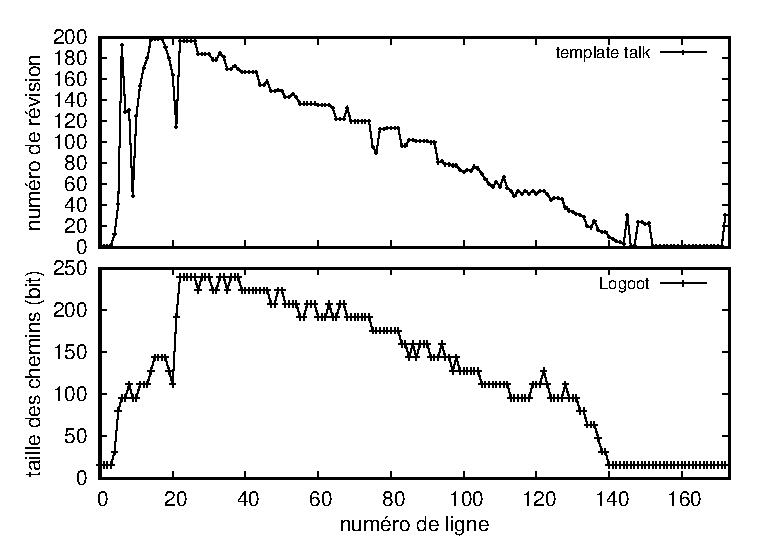
\includegraphics[width=0.8\textwidth]{img/lseq/motivationlogoot.eps}
    \caption[Taille des chemins alloués par Logoot sur un document édité en
    tête]{\label{repl:img:motivationlogoot} Taille des chemins alloués par
      Logoot sur un document principalement édité en tête. L'axe des abscisses
      montre le numéro de la ligne dans le document. L'axe des ordonnées de la
      partie haute de la figure montre la révision à laquelle a été ajoutée la
      ligne. L'axe des ordonnées de la partie basse de la figure montre la taille
      du chemin alloué à une ligne.}
  \end{center}
\end{figure}

\noindent Logoot favorise, par son choix d'entier proche de l'identifiant
précédent la position d'insertion, les comportements d'édition où les éléments
sont insérés de gauche à droite. Toutefois, lorsque le comportement d'édition va
à l'encontre de cette stratégie, la taille des identifiants peut augmenter
extrêmement rapidement. La figure~\ref{repl:img:motivationlogoot} met en
évidence cette croissance. La taille des chemins (i.e. les identifiants uniques
de site et compteurs sont ignorés) augmente par pallier. De nombreuses séries
d'insertions en tête se traduisent par l'ajout d'un niveau dans les chemins. Sur
un petit document de moins de 200 lignes, un chemin alloué par Logoot atteint 16
concaténations. Ici, chacune de ces concaténations pèse 16 bits.  La complexité
spatiale de chaque identifiant est linéaire par rapport au nombre d'insertions dans
le document, et puisque chaque identifiant est disséminé aux autres répliques,
la complexité en communication adopte cette progression. De plus, les valeurs
choisies par Logoot dans les identifiants sont toujours comprises entre $0$ et
$2^{c}$ où $c$ est une constante ($c = 16$ dans la
figure~\ref{repl:img:motivationlogoot}). Cette constance implique que, même dans
le cadre du comportement d'édition attendu, la complexité est linéaire -- bien
que fortement atténuée. Là encore, le trafic généré en souffre directement.

\noindent La représentation de la séquence sous forme de liste possède
l'avantage de fournir un accès instantané à ses éléments. Ainsi, la traduction
de \og insérer l'élément $e$ à la position $i$ \fg à \og insérer l'élément $e$
ente l'identifiant $id_{i}$ de l'élément en position $i+1$ et l'identifiant
$id_i$ de l'élément en position $i$ \fg s'effectue en temps constant.
Cependant, cette rapidité d'accès est seulement possible au détriment d'une
consommation en espace élevée : Logoot ne profite pas de la redondance
d'information sur les triples. La complexité spatiale de la structure est
quadratique par rapport au nombre d'insertions effectuées dans la séquence.

\noindent Une extension nommée \textbf{Logoot split}~\cite{andre2013supporting}
étend Logoot lui offrant la possibilité d'adapter la granularité de l'élément
ciblé.  Cette extension prend pour granularité la chaîne de caractères avec la
liberté de la scinder si besoin est. Le nombre d'identifiants à allouer s'en
trouve diminué, et par conséquent, le trafic généré également. Cette
amélioration est orthogonale et s'applique à tous les CRDTs générant des
identifiants de taille variable.

\paragraph{Treedoc~\cite{letia2009crdts, preguica2009commutative} :} Cette
approche représente le document sous forme d'arbre binaire avec parcours infixe.
Lorsqu'il n'y a pas de concurrence, chaque nœud de l'arbre possède au plus un
élément et au plus 2 fils. Les arêtes de l'arbre sont étiquetées par la valeur
binaire 0 ou 1.  Si un nœud possède un élément et deux fils, tous les éléments
du sous-arbre accessible par l'arête dont l'étiquette est 0 se trouvent à gauche
de ce premier élément; tous les éléments du sous-arbre accessible par l'arête
dont l'étiquette est 1 se trouve à droite de ce premier élément. Du fait de la
concurrence, chaque nœud peut aussi devenir un super-nœud accueillant plusieurs
nœuds. De plus, chaque nœud est décoré d'un identifiant unique de site et d'un
compteur local à ce site. Ainsi, les nœuds contenus dans chaque super-nœud
suivent eux aussi un ordre total. Un identifiant est donc une liste de triples
$id = [t_1.t_2\ldots t_k]$ où $k$ est un entier, et
$t_k = \langle b_k,\, s_k,\, c_k\rangle$ où $b_k$ est une valeur binaire, $s_k$
est un identifiant unique de site, et $c_k$ est un compteur local au site $s_k$.
Prenons par exemple les éléments adjacents
$id_i=[\langle 0,\,s_1,\,c_1 \rangle.\langle 1,\,s_1,\,c_2 \rangle]$ et
$id_{i+1}=[\langle 0,\,s_1,\,c_1 \rangle.\langle 1,\,s_1,\,c_2 \rangle. \langle
1,\, s_2,\, c_3 \rangle]$.
Lors de la $x$\up{ème} insertion locale par le site $s_y$, Treedoc examine les
identifiants adjacents à la position d'insertion. Treedoc commence par examiner
si un identifiant est l'ancêtre direct de l'autre, i.e., la liste de triples
d'un identifiant est incluse dans la liste de triples de l'autre
identifiant. Par exemple, $id_{i}$ est l'ancêtre de $id_{i+1}$. Dans ce cas,
Treedoc copie l'identifiant du descendant et le suffixe par
$\langle 1,\, s_y,\, x \rangle$ si le descendant précède la position
d'insertion; $\langle 0,\, s_y,\, x \rangle$ dans le cas contraire. Si aucun des
identifiants n'est l'ancêtre de l'autre, Treedoc choisit de copier l'identifiant
précédant la position d'insertion et lui suffixe le triple
$\langle 1,\, s_y,\, x \rangle$.


\begin{figure}
  \begin{center}
    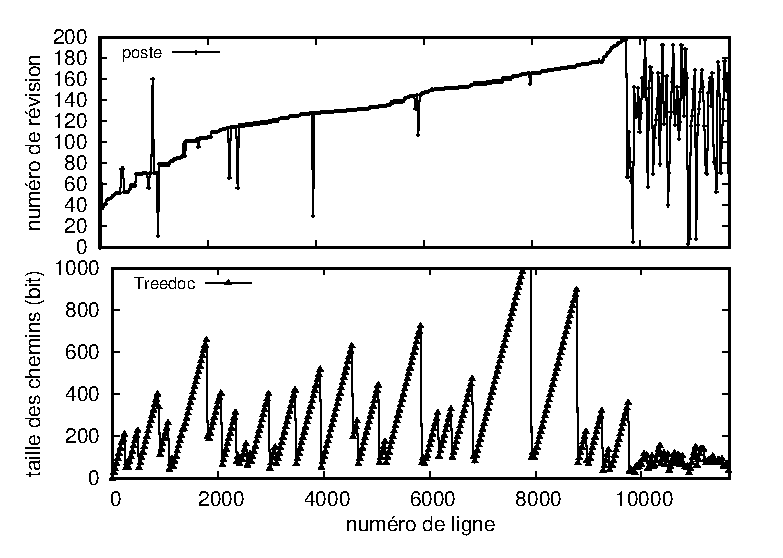
\includegraphics[width=0.8\textwidth]{img/lseq/motivationtreedoc.eps}
    \caption[Taille des chemins alloués par Treedoc sur un grand document édité
    en fin]{\label{repl:img:motivationtreedoc} Taille des chemins alloués par
      Treedoc sur un grand document principalement édité en fin. L'axe des
      abscisses montre le numéro de la ligne dans le document. L'axe des
      ordonnées de la partie haute de la figure montre la révision à laquelle a
      été ajoutée la ligne. L'axe des ordonnées de la partie basse de la figure
      montre la taille du chemin alloué à une ligne.}
  \end{center}
\end{figure}


\noindent La figure~\ref{repl:img:motivationtreedoc} met en évidence la
croissance rapide des chemins (i.e. les identifiants uniques de site et
compteurs sont ignorés) alloués par Treedoc. Un série d'insertions se succédant
conduit à des identifiants de plus de 1k bits. Tout comme l'approche Logoot, les
observations effectuées sur un corpus de documents Wikipédia montrent
l'importance d'une stratégie d'allocation gérant l'édition de gauche à
droite. Elles conduisent à proposer une heuristique selon laquelle des nœuds de
l'arbre sont virtuellement créés en prévoyance des éditions à venir. Toutefois,
de manière identique à Logoot, lorsque le comportement d'édition va à l'encontre
de cette stratégie, les identifiants sont de taille linéaire par rapport à la
taille du document.


\noindent La représentation de la séquence sous forme d'arbre possède l'avantage
de factoriser les nombreux triples communs composant les identifiants
Treedoc. Cette forme compacte de structure a le défaut de ne pas permettre
d'accès direct aux identifiants. Retrouver les identifiants adjacents à la
position d'insertion requiert un parcours de l'arbre. De plus, cette
représentation compacte n'a pas d'incidence sur les identifiants
eux-mêmes. Puisque chaque identifiant doit être disséminé individuellement aux
autres répliques, le trafic généré demeure inchangé par ce choix de structure.

Les CRDTs fonctionnant avec des identifiants de taille variable n'utilisent pas
de pierres tombales lors de la suppression d'éléments. Par conséquent, la
mémoire consommée par ces approches n'est pas strictement croissante. Un
document vide signifie que la séquence répliquée est également vide. En
revanche, les identifiants peuvent croître de manière linéaire par rapport au
nombre d'insertions dans le document. Malheureusement, cette progression se
répercute sur la complexité en communication. De même, cette progression se
répercute sur les performances à l'intégration des opérations d'insertion.

Une solution consiste à relocaliser les identifiants. En d'autres termes, les
identifiants sont modifiés au profit d'identifiants plus courts et conservant
l'ordre dense des éléments de la séquence. Toutefois, supprimer puis réinsérer
l'ensemble des éléments dans un document neuf ne suffit pas : le trafic engendré
est élevé et un tel processus effectué en concurrence est susceptible de cloner
les éléments. Il faut donc parvenir à prendre une décision globale sur la
relocalisation ce qui revient à obtenir un consensus en contexte réparti. Les
consensus sont coûteux à obtenir dans les systèmes à large échelle où le nombre
de répliques est grand, et particulièrement lorsque ces répliques ne sont pas
accessibles en permanence.

Afin d'éviter les baisses de performance ainsi que les mécanismes de
relocalisation, une autre solution consiste à obtenir des identifiants
suffisamment courts pour qu'ils ne nécessitent pas d'être relocalisé. La section
suivante s'attache à décrire les difficultés liées à l'allocation d'identifiants
à taille variable.

%%% Local Variables:
%%% mode: latex
%%% TeX-master: "../../paper"
%%% End:
